\documentclass[tikz, preview]{standalone}

\usepackage{amsfonts, amsthm, amssymb, amsmath, stmaryrd, etoolbox}
\usepackage{tikz}
\usepackage[all,2cell]{xy}
\usetikzlibrary{matrix,arrows,shapes,decorations.markings,decorations.pathreplacing}
\definecolor{rewritecolor}{rgb}{0,.9,1}
\tikzset{rewritenode/.style={shape=circle,fill=rewritecolor,scale=0.25,font=\Huge}}
\tikzset{RWopen/.style={shape=circle,draw=black,fill=white,scale=0.5,font=\Huge}}
\tikzset{RWclosed/.style={shape=circle,fill=black,scale=0.5,font=\Huge}}
\tikzset{CDnode/.style={shape=circle,fill=white,scale=.5}}
\tikzset{zxgreen/.style={shape=circle,draw,thick,fill=green}}
\tikzset{zxred/.style={shape=circle,draw,thick,fill=red}}
\tikzset{zxyellow/.style={shape=rectangle,draw,thick,fill=yellow}}
\tikzset{zxdiamond/.style={shape=diamond,fill=black,inner sep=2.75}}
\tikzset{zxopen/.style={shape=circle,draw,thick,inner sep=2pt}}
\tikzset{->-/.style={decoration={markings,mark=at position .5 with {\arrow{>}}},postaction={decorate}}}

\begin{document}
\[
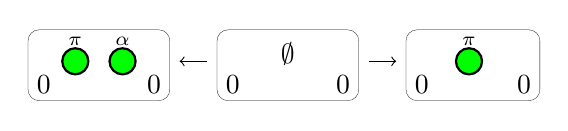
\begin{tikzpicture}
	%
	%
	%
	\begin{scope}[shift={(-4.8,-0.6)}]
	\node [zxgreen,label={[shift={(0,-0.1)}]\scriptsize $\pi$}] (v1) at (0.8,0) {};
	\node [zxgreen,label={[shift={(0,-0.1)}]\scriptsize $\alpha$}] (v2) at (1.4,0) {};
	%
	\node at (0.4,-0.3) {$0$};
	\node at (1.8,-0.3) {$0$};
	\node (v11) at (2,0) {};
	\draw [ultra thin, rounded corners] (0.2,0.4) rectangle (2,-0.5);
	\end{scope}
	%
	%
	%
	\begin{scope}[shift={(0.8,-0.1)}]
	\node at (-2.1,-0.4) {$\emptyset$};
	%
	\draw [ultra thin, rounded corners] (-3,-0.1) rectangle (-1.2,-1);
	\node at (-2.8,-0.8) {$0$};
	\node at (-1.4,-0.8) {$0$};
	\node (v12) at (-3,-0.5) {};
	\node (v14) at (-1.2,-0.5) {};
	\end{scope}
	%
	%
	%
	\begin{scope}[shift={(2.1,-0.8)}]
	\node [zxgreen,label={[shift={(0,-0.1)}]\scriptsize $\pi$}] (v6) at (-1.1,0.2) {};
	\node at (-1.7,-0.1) {$0$};
	\node at (-0.4,-0.1) {$0$};
	%
	\draw [ultra thin, rounded corners] (-1.9,0.6) rectangle (-0.2,-0.3);
	\node (v13) at (-1.9,0.2) {};
	\end{scope}
	%
	%
	%
	\draw [<-] (v11) edge (v12);
	\draw [<-] (v13) edge (v14);
\end{tikzpicture}
\]
\end{document}
